\documentclass[british,titlepage]{ntnuthesis}

\usepackage{listings-solidity} % copy listings-solidity.sty to your project

\usepackage{xcolor}
\definecolor{verylightgray}{rgb}{.97,.97,.97}

\lstset{ % define general preferences
	backgroundcolor=\color{verylightgray},
	extendedchars=true,
    showstringspaces=false,
    showspaces=false,
    tabsize=4,
}

\title{EduWallet: A Blockchain-Enabled Digital Wallet for Managing University Course Credits}
\shorttitle{EduWallet}
\author{Diego Da Giau}
\date{2025-05-01}

\addbibresource{thesis.bib}


% From https://www.overleaf.com/learn/latex/Glossaries

\makeglossaries % Prepare for adding glossary entries

\newglossaryentry{application programming interface}{
        name=Application Programming Interface,
        plural=application programming interfaces,
        description={A set of rules and protocols that allow different software applications to communicate with each other, enabling them to exchange information or functionalities}
}

\newglossaryentry{mempool}{
    name=mempool,
    plural=mempools,
    description={Short for memory pool. In general computing, it refers to a temporary memory area used to manage pending operations. In the context of blockchain and account abstraction, a mempool is a temporary storage area to hold UserOerations that have been broadcast to the network but are not yet included in a block}
}

\newglossaryentry{salt}{
    name=salt,
    plural=salts,
    description={A salt is a random sequence of data used in cryptography. It is added to a password before hashing, with the purpose of making the resulting hash unique, even if two users have the same password}
}

\newglossaryentry{keccak256}{
    name=Keccak-256,
    description={A cryptographic hash function that belongs to the Keccak family. It produces a fixed 256-byte hash},
}

\newglossaryentry{nonce}{
    name=nonce,
    plural=nonces,
    description={A nonce is a number that can be used only once in a cryptographic communication. In \acrlong{eth}, the nonce represents the number of transactions sent by a specific address and is used to ensure the uniqueness and validity of each transaction},
}

\newglossaryentry{hash}{
    name=hash,
    plural=hashes,
    description={In computer science, a hash function is an algorithm that takes an input of arbitrary length and produces a fixed-size output, commonly referred to as a hash or digest},
}

\newglossaryentry{double-spending}{
    name=double-spending,
    description={The double-spending problem refers to the malicious act of spending the same digital currency multiple times. In digital systems without adequate safeguards, this vulnerability could allow users to duplicate funds and undermine the integrity of the monetary system},
}

\newglossaryentry{p2p}{
    name=peer-to-peer,
    description={A peer-to-peer network is a distributed system architecture in which all participating nodes, called peers, have equal authority and responsibility},
}

% --------------------
% ----- Acronyms -----
% --------------------

\newacronym{ew}{EW}{EduWallet}
\newacronym{lms}{LMS}{Learning Management System}
\newacronym{api}{API}{\gls{application programming interface}}
\newacronym{sw}{SW}{Smart Wallet}
\newacronym{sdk}{SDK}{Software Development Kit}
\newacronym{cli}{CLI}{Command Line Interface}
\newacronym{ipfs}{IPFS}{InterPlanetary File System}
\newacronym{cid}{CID}{Content Identifier}
\newacronym{url}{URL}{Uniform Resource Locator}
\newacronym{ui}{UI}{User Interface}
\newacronym{gui}{GUI}{Graphical User Interface}
\newacronym{ux}{UX}{User Experience}
\newacronym{ects}{ECTS}{European Credit Transfer and Accumulation System}
\newacronym{eth}{ETH}{Ethereum}
\newacronym{evm}{EVM}{Ethereum Virtual Machine}
\newacronym{eoa}{EOA}{Externally Owned Account}
\newacronym{sca}{SCA}{Smart Contract Account}
\newacronym{it}{IT}{Information Technology}
\newacronym{abi}{ABI}{Application Binary Interface}
\newacronym{aws}{AWS}{Amazon Web Services}
\newacronym{pdf}{PDF}{Portable Document Format}
\newacronym{fr}{FR}{Functional Requirement}
\newacronym{nfr}{NFR}{Non-Functional Requirement}
\newacronym{www}{WWW}{World-Wide Web}
\newacronym{btc}{BTC}{Bitcoin}
\newacronym{dapp}{dApp}{decentralized application}
\newacronym{mit}{MIT}{Massachusetts Institute of Technology}
\newacronym{dcc}{DCC}{Digital Credential Consortium} % add glossary and acronym lists before document

\begin{document}

% \chapter*{Abstract}

% \chapter*{Sammendrag}
Mens verden raskt går fra tradisjonelle Web 2.0-systemer, dominert av store selskaper som tjener penger på sentraliserte data, til Web3-løsninger basert på blockchain-teknologiens desentraliserte natur, er akademia fortsatt i stor grad avhengig av sentraliserte databaser og statiske dokumenter, enten digitale eller på papir. Denne utdaterte tilnærmingen hindrer deling av akademiske opplysninger mellom institusjoner, som ofte krever produksjon, validering og verifisering av dokumenter, samt enighet om felles formater.

Dette arbeidet foreslår en løsning for å modernisere forvaltningen av akademiske opptegnelser. Ved å utnytte blockchain og Ethereum smart contracts legger vi grunnlaget for et system basert på sikre og manipulasjonssikre teknologier. Gjennom bruk av kontoabstraksjon er vi i stand til å utvikle en brukervennlig løsning som muliggjør gasless interaksjoner for brukerne. EduWallet er avhengig av et Software Development Kit (SDK) som gjør det mulig for universiteter å samhandle med on-chain-funksjonaliteter, og en nettleserutvidelse som gjør det mulig for studenter å administrere sine data. En viktig funksjon i den foreslåtte løsningen er full dataeierskap, som i sin helhet gis til studentene, som kontrollerer tilgangen til sine akademiske opplysninger. I tillegg brukes et desentralisert lagringssystem til å lagre studentenes sertifikater, noe som minimerer behovet for lagring av data på kjeden.

EduWallet har som mål å tilby et omfattende miljø innenfor akademiske institusjoner, slik at universitetene kan effektivisere byråkratiske prosesser og tilpasse seg de nyeste Web3-standardene. Den foreslåtte løsningen fungerer også som et praktisk eksempel på hvordan man effektivt kan integrere on-chain- og off-chain-komponenter i et sammenhengende system.

\tableofcontents
\listoffigures
\listoftables
\lstlistoflistings

\printglossary[type=\acronymtype] % Print acronyms
\printglossary                    % Print glossary

% \chapter{Introduction}
\label{chap:introduction}
We are currently living in a globalized world, where distance is increasingly irrelevant. People move freely across borders, and thanks to digital technologies, everyone is interconnected and can access services regardless of location. Schools and universities are deeply affected by this globalization, and their internal operations are rapidly evolving. Today, many students receive education from a variety of sources, often through online courses offered by institutions in different countries. 
A further driver of this change is the rise of academic mobility programs, such as the Erasmus program, an initiative by the European Union designed to promote student and faculty exchanges and foster intercultural experiences.

However, these opportunities introduce challenges in managing and sharing students' academic records. Typically, each university maintains its own format and system for storing academic data, which creates friction when this information needs to be exchanged. When a student transfers to another institution or participates in an exchange program, they must present verified academic documentation, including diplomas and course transcripts. Currently, students are required to request certified digital or paper documents from their home institution, which must be signed and validated by the university. They then submit these to the receiving institution, which must verify the authenticity of both the data and the signatures. This multi-step process is burdensome for both students and universities, involving significant administrative overhead and document handling.

Given our experience with the Erasmus exchange program, and the tedious process of requesting documentation, waiting for it, and resolving discrepancies between universities regarding content and validation, we decided to develop this project. The aim of this thesis is to provide both students and universities with a unified system for storing and sharing academic records. \gls{ew} leverages blockchain technology, utilizing its tamper-proof and verifiable nature to allow universities to securely issue academic records and certificates, while enabling students to access them through ownership of an academic wallet in which the records are stored. User interaction is a central focus of this work, as the solution is intended for students of all backgrounds, without requiring specific computer science skills. Therefore, the system is designed to abstract the complexity of its blockchain-based core.

The remainder of this document is structured as follows: the next chapter, \cref{chap:background}, provides the necessary background information on blockchain and the technologies used within \gls{ew}. \cref{chap:relatedWork} presents the related work. Based on the context established in the previous chapters, \cref{chap:problemStatement} explains the problem addressed in this thesis and introduces the use cases that guided the system design. \cref{chap:requirements} outlines the requirements derived from these use cases.
The design of the proposed solution is presented in \cref{chap:systemArchitecture}, which gives an overview of the components that make up \gls{ew}, and is further detailed in \cref{chap:onchainDesign} and \cref{chap:offchainDesign}, which describe the on-chain and off-chain elements, respectively. The tools and code used for the development of the system are discussed in \cref{chap:implementation}.
A discussion on the solution and the outcomes of this work is provided in \cref{chap:validation}. Finally, \cref{chap:conclusion}  concludes the thesis by summarizing its main contributions and \cref{chap:futureWork} presents directions for future research.
% \chapter{Background Material}
\label{chap:background}
The aim of this chapter is to provide the reader with the fundamentals concepts necessary to understand discussed in this work. All the background knowledge presented here is related to emerging decentralized technologies, which are leveraged to modernize the university system in line with Web3 paradigm.

The chapter begins by tracing the evolution of the internet and websites, from the earliest technologies to today's decentralized web. It then delves into blockchain technologies, with a particular focus on one of the most prominent platforms, \acrlong{eth}. The final section explores decentralized storage solutions, which serve as a bridge between fully on-chain systems and traditional web-based services.

%%%%%%%%%%%%%%%%%%%%%%%%%%%%%%%%%%%%%%%%%%%%%%%%%%%%%%%%%%%%%%%%%%
% FROM WEB 1.0 TO WEB3
%%%%%%%%%%%%%%%%%%%%%%%%%%%%%%%%%%%%%%%%%%%%%%%%%%%%%%%%%%%%%%%%%%
\section{From Web 1.0 to Web3}
The \acrfull{www} \cite{berners1992world} was launched in 1991 with the publication of the first website\footnote{\url{https://info.cern.ch/}} by the English computer scientist Tim Berners-Lee. The goal behind the \acrshort{www} was to create a digital archive of collective human knowledge, accessible to anyone, everywhere. The first iteration of the web is known as Web 1.0, that was composed primarily of static web pages \cite{choudhury2014world}, where users' main activities were limited to reading content created by technically skilled individuals or interacting via emails and chat rooms \cite{murray2023promise}. A major limitation of this model was the stateless nature of protocols like HTTP, which prevented websites from storing or recall user data. As a result, web pages were static and offered limited interactivity, making them unattractive for commercial purpose since monetization was difficult.

Web 2.0 emerged to address these issues by introducing dynamic websites to the \acrshort{www}. In the early 1990s, Lou Montulli, a developer at Netscape, introduced browser cookies \cite{kristol1997rfc2109}, small data files stored by web pages to retain user information. This innovation enabled websites to become dynamic, offering personalized experiences based on user behaviour and preferences. It also paved the way for monetization, as companies could now track and analyse their data. Web 2.0 gave rise to modern tech giants such as Google and Microsoft, whose business models heavily rely on collecting and leveraging user data. However, this shift led to a new issue: user data became the property of centralized platforms, which could exploit or sell it without users' consent.

Web3 aims to reverse this trend by decentralising data ownership and returning control to the users \cite{sheridan2022web3}\cite{ray2023web3}. In the Web3 paradigm, individuals can own their data and choose how it is shared or monetized. The core technology enabling this transformation is the blockchain, a distributed ledger that facilitates interactions with digital services without relying on centralized structures.

%%%%%%%%%%%%%%%%%%%%%%%%%%%%%%%%%%%%%%%%%%%%%%%%%%%%%%%%%%%%%%%%%%
% BLOCKCHAIN
%%%%%%%%%%%%%%%%%%%%%%%%%%%%%%%%%%%%%%%%%%%%%%%%%%%%%%%%%%%%%%%%%%
\section{Blockchain}
A blockchain \cite{nofer2017blockchain} is a linked structure composed of data packages called blocks (hence the name blockchain). Each block contains multiple operations, known as \textit{transactions}, along with metadata such as the cryptographic \gls{hash} of the previous block. This structure links each block to its predecessor, forming the chain depicted in \cref{fig:blockchainStructure}, ensuring the integrity of the entire ledger. Since each block includes the \gls{hash} of the previous one, tampering with a block would require altering all the subsequent blocks in the chain, making such modifications computationally infeasible. 

\begin{figure}
  \centering
  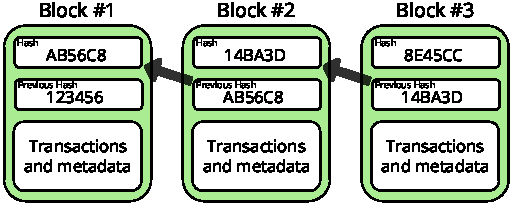
\includegraphics[width=0.7\textwidth]{figures/blockchain.pdf}
  \caption[Blockchain structure]{Blockchain structure showing the chain of blocks.}
  \label{fig:blockchainStructure}
\end{figure}

Blockchains are typically maintained by a \gls{p2p} network, where each participant, referred to as \textit{node}, stores a copy of the blockchain. This decentralized replication ensures data availability, fault tolerance, and security. Nodes follow a consensus protocol, which defines the rules by which transactions are validated and blocks are added to the chain. 

The first blockchain was introduced in 2008 by Satoshi Nakamoto, the pseudonymous creator (or group of creators) of Bitcoin \cite{nakamoto2008bitcoin}. It continues to function as the public ledger for all \acrlong{btc} transactions, effectively solving the \gls{double-spending} problem without the need for a centralized authority. Another widely known blockchain is \acrfull{eth}, which operates alongside its native cryptocurrency, Ether.

%%%%%%%%%%%%%%%%%%%%%%%%%%%%%%%%%%%%%%%%%%%%%%%%%%%%%%%%%%%%%%%%%%
% ETHEREUM
%%%%%%%%%%%%%%%%%%%%%%%%%%%%%%%%%%%%%%%%%%%%%%%%%%%%%%%%%%%%%%%%%%
\section{Ethereum}
\acrlong{eth}\footnote{\url{https://ethereum.org}} was launched in 2015 based on an idea of Vitalik Buterin \cite{buterin2014next}\cite{wood2014ethereum}. Buterin's vision was to enable the deployment of \acrfull{dapp}, programs that run autonomously on a blockchain without relying on external, centralized infrastructure. To realize this vision, he and his collaborators created the \acrfull{evm}, a decentralized virtual machine that executes transactions. In contrast to \acrlong{btc}'s limited instruction set, the \acrshort{evm} supports a broad range of operations, including loops and conditional statements. This flexibility makes it possible to develop \textit{smart contracts}, which are programs containing both code and data that execute on the \acrlong{eth} blockchain.

When users perform on-chain operations, such as sending cryptocurrency or invoking a smart contract function, they consume computational resources. To compensate nodes for providing these resources and to prevent abuse (for example, infinite loops), Ethereum measures resource usage in units called \textit{gas}. Each individual operation requires a specific amount of gas, and the total \textit{gas fee} for a transaction is calculated by multiplying the gas used by the current \textit{gas price}. Because gas is paid in Ether, the cost of executing an operation varies with the market value of Ether.

Users hold Ethers and pay transaction fees via \acrfull{eoa}, which can initiate transactions and serve as the interface between users and the blockchain. An \acrshort{eoa} is derived from a private key, which is also required to cryptographically sign transactions. The other account type in Ethereum is the \textit{contract account}, which corresponds to a deployed smart contract. Contract accounts can hold cryptocurrency but cannot initiate transactions on their own; they can only send transactions in response to receiving one. Both contract accounts and \acrshort{eoa}s are publicly referenced by their address, which serves as the identifier used to send funds or invoke contract functions.

Due to its versatility and the wide range of operations it supports, \acrlong{eth} has become the foundation for numerous Layer 2 solutions \cite{sguanci2021layer2blockchainscaling} over time. Layer 2 solutions are protocols built on-top of the main blockchain (Layer 1) to provide additional features, such as an increased transaction throughput or reduced fees. The core idea behind these solutions is to process transactions off-chain and periodically submitting a summary about them on the Layer 1 chain. Some notable examples of \acrshort{eth} Layer 2 solutions are:

\begin{itemize}
    \item \textit{Polygon}\footnote{\url{https://polygon.technology}}, which offers faster and cheaper transactions compared to the \acrlong{eth} main network.
    \item \textit{Arbitrum}\footnote{\url{https://arbitrum.io}} \cite{kalodner2018arbitrum}, that enhances scalability while preserving compatibility with Ethereum smart contracts.
    \item \textit{ZKsync}\footnote{\url{https://www.zksync.io}}, a solution that ensures high security and fast finality through the use of validity proofs.
    \item \textit{Optimism}\footnote{\url{https://www.optimism.io}}, which prioritizes simplicity and close integration with the Ethereum ecosystem.
    \item \textit{Starknet}\footnote{\url{https://www.starknet.io}}, that introduces its own high-performance language, Cairo\footnote{\url{https://www.cairo-lang.org/}}.
\end{itemize}

%%%%%%%%%%%%%%%%%%%%%%%%%%%%%%%%%%%%%%%%%%%%%%%%%%%%%%%%%%%%%%%%%%
% DECENTRALIZE STORAGE
%%%%%%%%%%%%%%%%%%%%%%%%%%%%%%%%%%%%%%%%%%%%%%%%%%%%%%%%%%%%%%%%%%
\section{Decentralized Storage}
Since blockchain operations consume gas, and gas costs are significantly higher than those in traditional Web 2.0 solutions, especially for storage \cite{surya2024designdecentralizedidentity}, \acrshort{dapp}s often rely on decentralized storage solutions to handle large amounts of data and high-volume files \cite{ray2023web3}\cite{muhle2018survey}. These solutions distribute data across the nodes in the network, in contrast to traditional storage approaches that depends on centralized data centres.

One widely adopted decentralized storage system is \acrfull{ipfs} \cite{benet2014ipfscontentaddressed}, a protocol built on a \gls{p2p} network architecture, similar to blockchains. When users upload a file to \acrshort{ipfs}, it is assigned a unique identifier called a \acrfull{cid}, which corresponds to the \gls{hash} of the file's content \cite{erikflorian2022ipfsandfrineds}. Files can be replicated across multiple nodes to enhance availability and security.  To retrieve a file, users must use its \acrshort{cid} to locate and access the nodes storing it. This content-addressed design ensures file integrity and verifiability, as any change to the file would produce a new \acrshort{cid}.
% \chapter{Related Work}

% \chapter{Problem Statement}

% \chapter{Running Example}

\chapter{Requirements}
\label{chap:requirements}
In this chapter, our aim is to describe both the functional and non-functional requirements that guided us in the development of the comprehensive academic wallets system. These requirements are summarized in \cref{tab:funcReq} and \cref{tab:nonFuncReq}, respectively. They were derived from an in-depth analysis of the use cases, as well as the specific needs and demands of the various stakeholders engaged with the system. This stakeholder group includes the administrator of the \acrfull{ew} system, students, and universities.

%%%%%%%%%%%%%%%%%%%%%%%%%%%%%%%%%%%%%%%%%%%%%%%%%%%%%%%%%%%%%%%%%%
% FUNCTIONAL REQUIREMENTS
%%%%%%%%%%%%%%%%%%%%%%%%%%%%%%%%%%%%%%%%%%%%%%%%%%%%%%%%%%%%%%%%%%
\begin{table}[htpb]
\centering
\caption{Functional Requirements}
\label{tab:funcReq}
\begin{tabular}{|p{1.0cm}|p{11cm}|}
\hline
\multicolumn{2}{|c|}{\textbf{System Administration}} \\
\hline
FR1 & Allow the system administrator to verify and approve universities requesting access to the \acrlong{ew} system. \\
\hline
\multicolumn{2}{|c|}{\textbf{University}} \\
\hline
FR2 & Enable universities to register and subscribe to the system. \\
FR3 & Provide secure authentication mechanisms for universities to access the platform. \\
FR4 & Allow universities to create new smart contract wallets for students upon enrolment. \\
FR5 & Enable universities to read from and issue academic records to students' smart wallets. \\
FR6 & Implement authorization controls to ensure that only permitted universities can access or modify specific academic records. \\
FR7 & Provide a mechanism for universities to request and obtain permission from students before accessing or modifying their academic records. \\
FR8 & Provide APIs that allow universities to integrate the \acrlong{ew} system with their existing \acrlong{lms}. \\
\hline
\multicolumn{2}{|c|}{\textbf{Student}} \\
\hline
FR9  & Students must own and manage their academic smart wallets independently. \\
FR10 & Enable students to securely authenticate and access their smart wallets. \\
FR11 & Provide students with a web-based interface to view and manage their academic records. \\
FR12 & Allow students to grant and revoke access permissions to their academic records for specific institutions. \\
\hline
\end{tabular}
\end{table}
\section{Functional Requirements}
The primary functional requirement for the system administrator is the ability to register universities following their subscription request. This process must be preceded by a thorough verification of the provided data, in order to ensure that only trusted institutions are granted access to the system. The validation step is fundamental, as universities are the entities entitled to register new students in the academic record. Consequently, if malicious actors are authorized to access the system, its security and the veracity of the stored data could be compromised.

Regarding universities, they must be able to initiate a subscription by submitting their institutional information, including name and country. Upon approval, they require secure authentication mechanisms to access the system and exercise their privileges. Authentication is a critical precondition for nearly all operations, including the viewing and modification of students' data and academic records. These operations may involve retrieving the list of courses attended by a student or issuing a new certification. Furthermore, authenticated universities are responsible for creating \acrfull{sw} for newly enrolled students who do not yet posses one, as well as requesting permission from students to access their existing wallets. Delegating the creation of student \acrshort{sw} to universities accelerates the data verification process, as the system relies on the institution's trustworthiness to validate student information. Academic records are strictly personal data and must be handled with extreme caution. For this reason, without proper authentication, access to student, whether for viewing or modification, must be strictly restricted. 
Finally, since blockchain technologies can be difficult to interact with, due to their relatively recent development, the system should expose comprehensive \acrfull{api} endpoints. These can support seamless integration with university \acrfull{lms}, enabling them to interact with and utilize the full rage of fratures offered by \acrlong{ew}.

Students' functional requirements are closely aligned with the core principles of Web3 ownership: students must retain full control over their academic wallets. Consequentially, the \acrshort{ew} system must enable students to securely authenticate and access their \acrshort{sw} via a web interface, which also provides the ability to view and administer their data. A web application eliminates the need to install dedicated software on user devices and ensures a smoother multi-device experience.
Once authenticated, students should be able to grant universities explicit permissions to access their records, with fine-grained control over viewing and modification rights. This distinction is essential to manage different scenarios appropriately. For example, in the context of an exchange program, the host university should only be allowed to access a student's academic records, and not modify them.

%%%%%%%%%%%%%%%%%%%%%%%%%%%%%%%%%%%%%%%%%%%%%%%%%%%%%%%%%%%%%%%%%%
% NON-FUNCTIONAL REQUIREMENTS
%%%%%%%%%%%%%%%%%%%%%%%%%%%%%%%%%%%%%%%%%%%%%%%%%%%%%%%%%%%%%%%%%%
\begin{table}[htpb]
\centering
\caption{Non-Functional Requirements}
\label{tab:nonFuncReq}
\begin{tabular}{|p{1.0cm}|p{11cm}|}
\hline
NFR1 & The system shall operate without dependency on third-party wallet providers such as MetaMask. \\
NFR2 & The system shall minimize reliance on third-party technologies to enhance security and maintain control. \\
NFR3 & On-chain storage costs shall be minimized by storing only essential data, excluding large files. \\
NFR4 & Academic records shall be tamper-proof and verifiable by authorized third parties. \\
NFR5 & The system shall provide an intuitive and user-friendly interface for both students and university administrators. \\
NFR6 & The system architecture shall be designed to maximize decentralization wherever feasible. \\
\hline
\end{tabular}
\end{table}
\section{Non-Functional Requirements}
\label{sec:nonFunctionalRequirements}
In addition to the presented core features, the system must fulfil several non-functional requirements that ensure robustness, maintainability and alignment with the principles of decentralization. 

To preserve its independence, \acrshort{ew} must avoid reliance on third-party cryptocurrency wallets, such as MetaMask or Coinbase, as well as on proprietary technologies. These constraints are essential to prevent external dependencies that could compromise the system’s availability or security due to changes in external policies or services.

A key consideration for blockchain-based systems is the cost associated with on-chain storage operations \cite{surya2024designdecentralizedidentity}. To address this, the system must minimize blockchain storage usage by storing only essential data directly on-chain, while leveraging alternative technologies to manage and store files.

Academic records, by nature, must be verifiable and resistant to unauthorized modifications. The system must ensure that these records are temper-proof and can be verified by third parties at any time, in alignment with the integrity requirements of academic data.

Simplicity and ease of use are also critical. Since our target users are not necessary experts in blockchain or, more generally, in computer technologies, the system must offer an intuitive means of accessing and managing academic data. As such, both universities and students must be supported with a user-friendly interface that facilitates seamless interaction with the \acrshort{ew} platform.

Finally, the adoption of blockchain technologies is driven by the desire to embrace the defining characteristic of Web3 applications: decentralization. \acrshort{ew} should be designed to operate as a decentralized system, thereby avoiding the limitations and risks associated with centralized architectures, such as data security vulnerabilities, scalability constraints, and privacy concerns. % TODO: talk about Web3 and the advantages of decentralized systems over centralized ones.


\section{Constraints and Assumptions}
The system operates under the assumption that the user authentication phase is not the primary focus of the project. Therefore, it is sufficient to implement a basic mechanism to identify users and grant them access to their respective privileges. A key requirement is that this method be easily replaceable or upgradable, allowing for future integration of more sophisticated authentication solutions.

As the system is intended to serve as a Web3 extension for traditional \acrshort{lms} platforms, a critical constraint is that all on-chain operations must remain within acceptable gas limits. This ensures that blockchain transactions linger affordable and practical for real-world use. It is also assumed that universities and their technical staff possess a fundamental understanding of blockchain technologies, including key concepts such as wallets and transaction. This baseline knowledge is essential for effectively utilize the \acrshort{api} provided by \acrshort{ew}.
\chapter{Design}
To address the requirements presented in \cref{chap:requirements}, we developed a system composed of several components, as illustrated in \cref{fig:baseArchDiag}
and more in detail in \cref{fig:fullArchDiag}:
\begin{itemize}
    \item A set of \textit{smart contracts} responsible for all blockchain-related operations, including \acrshort{sw} creation and transaction management.
    \item A \textit{browser extension} that allows students to manage their academic wallets.
    \item A \textit{\acrfull{sdk}} designed for universities to interact with the \acrshort{ew} system.
    \item An external \textit{decentralized storage system} used to store and retrieve certification files (see \cref{sec:decStorageDesgn}).
\end{itemize}
\begin{figure}[htpb]
  \centering
  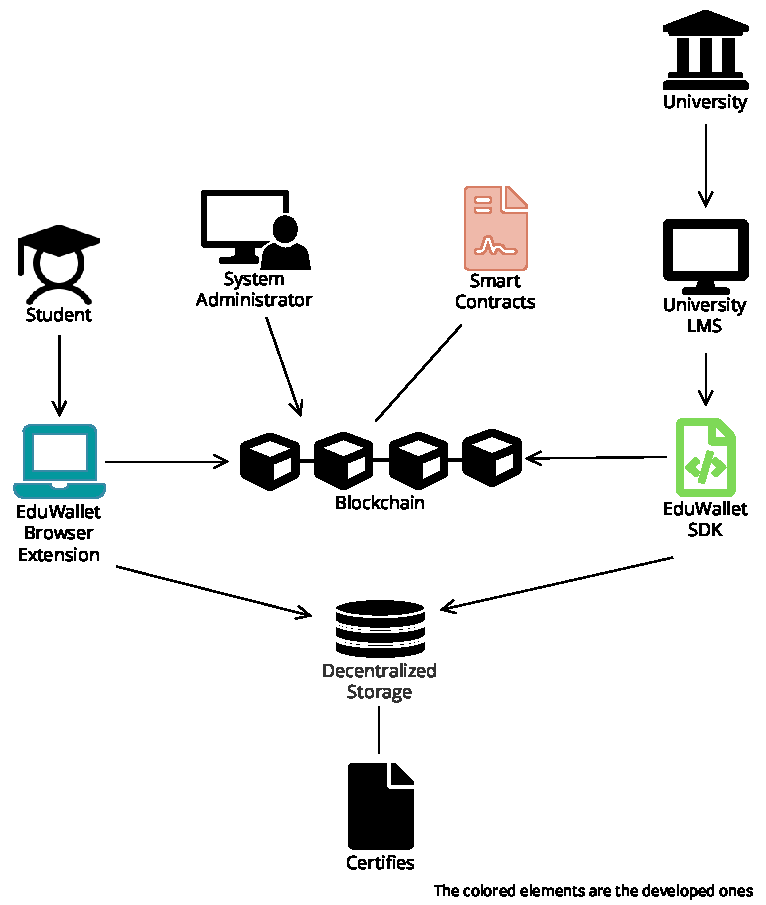
\includegraphics[width=0.5\textwidth]{figures/Architecture diagram basic.pdf}
  \caption[System basic architecture diagram]{The diagram shows the base architecture of the \acrlong{ew} system.}
  \label{fig:baseArchDiag}
\end{figure}

In addition to these core components, we developed a simple yet complete \textit{\acrfull{cli}}, which simulates a university's \acrshort{lms} and its interaction with the academic records system. The \acrshort{cli} serves as a testing and demonstration tool and enables users to perform all operations typically available to universities, thereby simplifying the interaction with our \acrshort{sdk}.

Since the focus of our work is on the interaction of universities and students with the academic registry, the system administrator's core functionality\footnote{The approval and subscription of universities} have been inserted directly in the \acrshort{cli}. This design decision streamlines our use case and reduces unnecessary complexity.

A more detailed analysis of each component is provided in the following sections.

\begin{figure}[htpb]
  \centering
  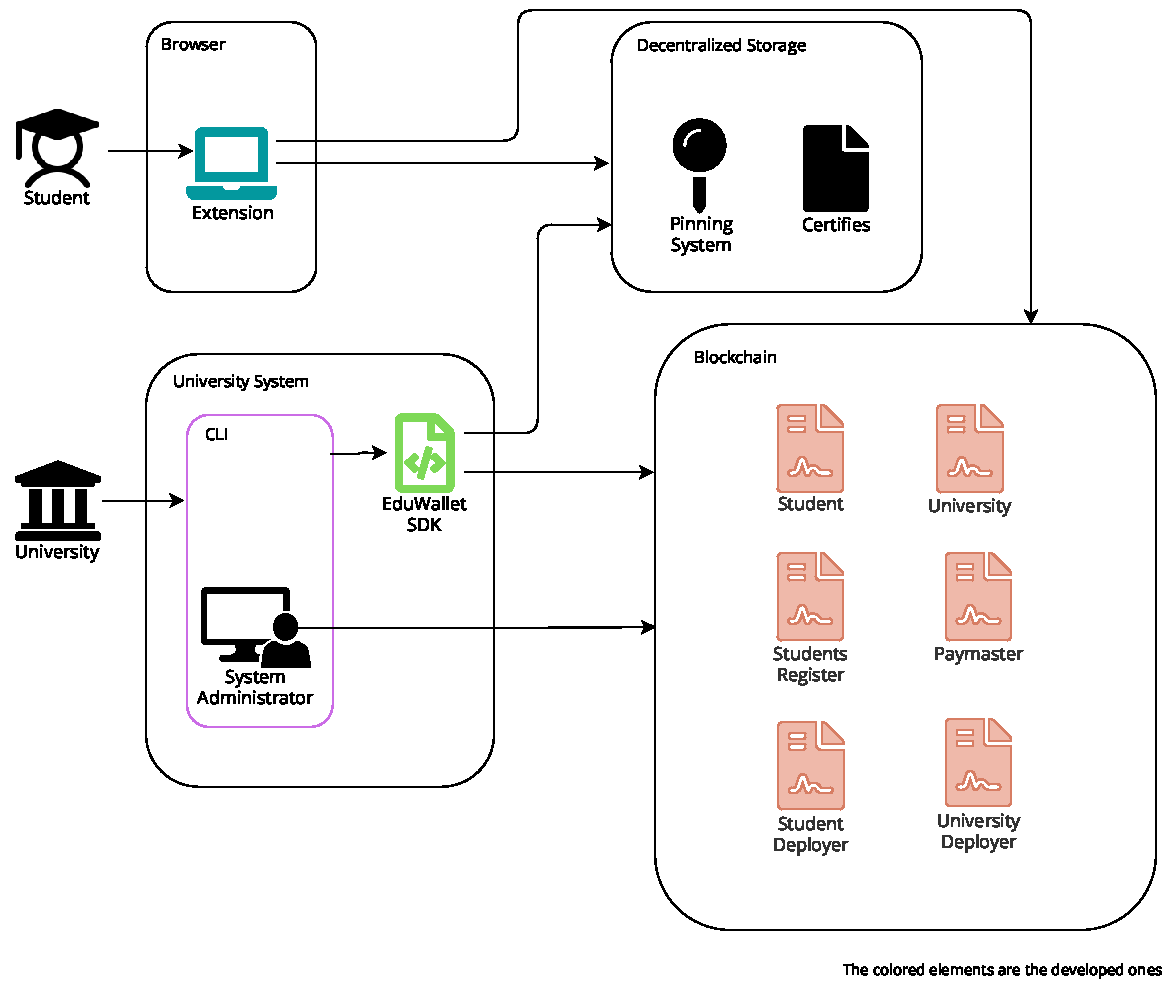
\includegraphics[width=0.7\textwidth]{figures/Architecture diagram complete.pdf}
  \caption[System architecture diagram]{The diagram shows the entire architecture of the \acrlong{ew} system.}
  \label{fig:fullArchDiag}
\end{figure}

\section{Smart Contracts}
\label{sec:smartContractsDesign}

\section{Browser Extension}
\label{sec:browserExtensionDesign}

\section{Decentralized Storage System}
\label{sec:decStorageDesgn}
To overcome one of the most significant challenges in blockchain systems, the cost of on-chain storage, we introduce an off-chain decentralized storage solution in our project. This system is used to store and retrieve certification files, such as language certificates or graduation diplomas, which require significantly more space than plain text\footnote{PDF files typically range from a few kilobytes to several megabytes, whereas plain text data usually occupies only a few bytes.}. Storing such documents directly on-chain would result in substantial gas costs, making the approach impractical. 

\subsection{Why a decentralized storage?}
We chose a decentralized storage system over traditional local or cloud-based solutions to maintain the decentralized nature of our environment and to meet the non-functional requirements outlined in \cref{sec:nonFunctionalRequirements}. Among the various decentralized options available, we selected \acrfull{ipfs} for its ability to provide verifiable and distributed file storage. This choice is motivated by several factors: \acrshort{ipfs} is an open source protocol with a large and active community, strong support, and widespread adoption. It also serves as the foundational layer for many other decentralized platforms, such as Filecoin\footnote{\url{https://filecoin.io}} and Web3.Storage\footnote{\url{https://web3.storage}}, allowing future extensions or upgrades to be implemented with minimal effort \cite{erikflorian2022ipfsandfrineds}. Furthermore, \acrshort{ipfs} ensures immutability of stored files, a critical feature for academic certificates, which must remain unchanged over time.

\subsection{Pinning files}
To fully leverage \acrshort{ipfs}, we integrated Filebase\footnote{\url{https://filebase.com}}, a third-party pinning service. Pinning refers to the act of instructing a node to keep a copy of a file permanently, preventing it from being removed during garbage collection. Without Filebase, we would have needed to run our own local \acrshort{ipfs} node and manage file pinning manually, an approach that introduces instead complexity, higher maintenance costs, and reduced data availability in a testing system like ours. In contrast, Filebase handles node operation and file pinning, offering an accessible solution thorough its AWS S3-compatible \acrshort{api}, which simplifies file uploads to the peer-to-peer network. Notably, Filebase also provides a free tier allowing up to 5 GB of storage, which is sufficient for our needs. This is an advantage over other pinning solutions such as Web3.Storage, which lacks a fully free plan, or Pinata\footnote{\url{https://pinata.cloud}}, which offers more limited options.

\subsection{Integration in the system}
As shown in \cref{fig:fullArchDiag}, both the browser extension and the \acrshort{sdk} interact with the storage system. The browser extension retrieves certificate associated with academic records using the official \acrshort{ipfs} public gateway. It presents students with a direct link to each certificate, composed by the gateway's base \acrshort{url} followed by the file's \acrfull{cid} on the \acrshort{ipfs} network. The \acrshort{cid} of each document is stored on-chain within the student's academic wallet, alongside other record information such as the course name. This enables students to view and download their certificates from a standard web interface.

% TODO: Add photo of the extension where you can see the link of a certification
Similarly, the \acrshort{sdk} uses the same mechanism to retrieve certificates on behalf of universities. When uploading a file, however, the \acrshort{sdk} interacts directly with Filebase to ensure the file is pinned and hosted by an active node. The \acrshort{sdk} receives the document from the university, then uses the AWS S3-compatible \acrshort{api} to upload it. The \acrshort{api} requires the key associated with the pinning account (managed by the \acrshort{ew} system administrator) and the file itself. In return, it provides the \acrshort{cid}, which is then stored in the academic record.
% TODO: Reference implementation section

\subsection{Security and Limitations}
Academic certifies, and official documents more broadly, are legal artifacts that must always be secure and verifiable. \acrshort{ipfs} inherently supports these properties through its use of content-based addressing. In this model, each file is identified by a \acrshort{cid}, which is derived from the cryptographic hash of the file's content. Any alteration to the file results in a completely different \acrshort{cid}, ensuring that tampering is immediately detectable \cite{benet2014ipfscontentaddressed}. Since the the \acrshort{cid} is stored on the blockchain at the time the certificate is issued by the university, the document's authenticity and integrity are guaranteed.

While \acrshort{ipfs} offers strong immutability and verifiability, it lacks built-in access control. In the context of our system, we assume that certificates are publicly accessible documents. Consequently, any part in possession of a file's \acrshort{cid} can retrieve it via the public gateway. However, if access control becomes a requirement, there are several strategies to address this limitation \cite{barbaraanrealaura2021datapersistence}. One option is to encrypt files before uploading them to \acrshort{ipfs}, such that only authorized components within our system can decrypt them. Another approach is to use a private \acrshort{ipfs} network, where access can be restricted to approved entities. The trade-offs and potential implications of such private deployment will be discussed in the FUTURE WORK CHAPTER.

\section{\acrshort{cli}}
\label{sec:cliDesign}

\chapter*{\bibname}
\printbibliography[heading=none]

\appendix
\chapter{GitHub Repository}
\label{chap:gitHub}

\url{https://github.com/NTNU-IDI/eduwallet-eduwalletdiego}
\chapter{Figma Prototype Link}
\label{chap:figma}

\url{https://www.figma.com/design/aZrmR2thWfRGKQWDQbZE9C/EduWallet?node-id=125-95&t=gQwA5a4uDzRy8jBl-1}
\chapter{Base Paymaster Contract}
\label{chap:basePaymaster}

\lstinputlisting[%
    caption={BasePaymaster smart contract},
    language=Solidity,
    numbers=left,
]{listings/BasePaymaster.sol}

\end{document}
